\documentclass[nfss,times,12pt,a4paper]{article}
\usepackage{epsfig}
\usepackage{times}
\usepackage{rotate}
\usepackage{graphicx}
	
\title{ Evolution of {\Huge{\bf{ \sc GiGa}}}\footnote{%
The document available at {\tt \$GIGAROOT/doc/GiGaEvolution.ps}}}
\author{ I.Belyaev\footnote{\tt E-mail: Ivan.Belyaev@itep.ru} \\
{\it ITEP (Moscow) }}
\begin{document}
\maketitle 

\abstract{
Several variants of evolution of 
{\sc GiGa}\footnote{%
See {\tt \$GIGAROOT/doc/GiGa.ps}} are discussed. 
The proposed schema for communications of 
algorithms within ${\mathcal{GAUDI}}$ framework 
with {\it Geant4} structures allows to use 
{\it Geant4 Tool Kit} as black-box without 
detailed knowledge of internal 
features of {\it Geant4 Tool Kit}.}

\tableofcontents 

 	
\section{ Integration of {\it Geant4} into ${\mathcal{GAUDI}}$ framework} 

The Evolution of {\sc GiGa} from stand-alone {\it Geant4} program 
to a simulation environment fully integrated into ${\mathcal{GAUDI}}$ 
framework could be represented by a set of phases and schematic diagrams 
of data flows. All indicated data flows consist of objects, specific for 
{\it Geant4 Tool Kit}. 

 
\subsection{ Phase~0  } 

Phase~0 corresponds to a stand-alone {\it Geant4} program. 
Data flows are schematically represented in figure~\ref{figOne}. 

\begin{figure}[ht] 
\setlength{\unitlength}{1mm} 
\begin{picture}(120,50)
\put(30,0){
\epsfig{file=GiGa_0_m.ps,%
height=50mm,%
bbllx=0pt,bblly=60pt,bburx=590pt,bbury=510pt,clip=}
}
\end{picture} 
\label{figOne} 
\caption{ A schematic view of {\it communications} with {\it Geant4 Tool Kit}.
Data flow directions are indicated by arrows. }
\end{figure} 



\subsection{ Phase~I  } 

At this phase we foreseen the 
introduction of {\sc GiGa} {\it Service} and 
the direct usage of this {\it service}
and some limited number of 
{\it Geant4} classes 
by {\it user}'s  {\it Algorithm}s. 
Data flows are schematically represented in figure~\ref{figTwo}. 


\begin{figure}[ht] 
\setlength{\unitlength}{1mm} 
\begin{picture}(120,100)
\put(10,0){
\epsfig{file=GiGa_1v1_m.ps,%
height=100mm,%
bbllx=0pt,bblly=60pt,bburx=590pt,bbury=660pt,clip=}
}
\end{picture} 
\label{figTwo} 
\caption{ A schematic view of data flows during Phase~I
of integration of {\it Geant4} into ${\mathcal{GAUDI}}$ framework}
\end{figure} 

This case corresponds to a native 
usage of "stand-alone" {\it Geant4} application 
within ${\mathcal{GAUDI}}$ framework. 
{\it User}'s algorithms act like wrappers over 
main program of {\it Geant4}.  
Frankly speaking at very beginning the only 
one profit that ordinary user gets from 
usage {\sc GiGa} Service with respect to 
an ordinary "stand-alone" {\it Geant4} program, 
is the fast and easy access to general and 
technical  ${\mathcal{GAUDI}}$ facilities 
like histogram, code profiling and others.  
 On other side, if one has the working 
{\it Geant4} code, it could be embedded into 
${\mathcal{GAUDI}}$ framework 
using {\sc GiGa} facilities in a straightforward 
way without changing 
any line of codes\footnote{Only the {\tt main() } function is to be removed}. 
   
Data flows between {\it Algorithm} and {\sc GiGa} {\it Service} 
indicated in figure~\ref{figTwo} still contain objects specific for 
{\it Geant4 Tool Kit}. 
 

\subsection{ Phase~II  }
 
This phase could be considered as 
{\it "transition phase"}  between Phase~I and Phase~III and 
it could be easily subdivided into some steps:

\begin{enumerate} 
\item 
At this step we enhance the functionality 
of {\sc GiGa} by making possible to extract the 
event record  from ${\mathcal{GAUDI}}$ {\it tvent store} 
\item 
At this step we enhance the functionality 
of {\sc GiGa} by making possible to get the 
Detector Description by pointing into the root of 
already constructed {\it Geant4} tree 
\item 
At this step we foreseen to implement the automatic
translation of ${\mathcal{GAUDI}}$ Detector 
Description into {\it Geant4} detector description.  
\item 
At this step we foreseen to implement the automatic
creation of {\it Geant4 hits} and {\it sensitive volume}
from their description via XML. A some common 
brainstorming within close collaboration with 
sub-detector groups is necessary for performing of 
this step.    
\item 
At this step we foreseen to automatic
translation of {\it Geant4 hits} into 
${\mathcal{GAUDI}}$ Monte Carlo objects\footnote{Obviously this step could not be done without close collaboration with sub-detector groups}
\item 
At this step we foreseen the automatic
population of ${\mathcal{GAUDI}}$ {\it event store} by information from 
 {\it Geant4 trajectories}\footnote{Communications physics and generator groups are required}
\end{enumerate} 
 
The data flows at the end of Phase~II are presented in figure~\ref{figThree}.
All input and output data flows from {\it Algorithm}s consist of only
${\mathcal{GAUDI}}$ specific objects. An intermediate layer of 
{\it Converter}s an d{\it conversion services} prevents any contacts between
{\it Algorithm}s and objects, specific for {\it Geant4}. 
One sees that now {\sc GiGa} {\it Service} itself 
becomes an internal and invisible object for ordinary user.

In addition one could foreseen the existence of intermediate sub-phase, 
sketched in figure~\ref{figFour}.  

\begin{figure}[ht] 
\setlength{\unitlength}{1mm} 
\begin{picture}(120,120)
\put(10,0){
\epsfig{file=GiGa_2v3_m.ps,%
height=120mm,%
bbllx=0pt,bblly=50pt,bburx=590pt,bbury=810pt,clip=}
}
\end{picture} 
\label{figThree} 
\caption{ A schematic view of data flows at the end of Phase~II
of integration of {\it Geant4} into ${\mathcal{GAUDI}}$ framework}
\end{figure} 



\begin{figure}[ht] 
\setlength{\unitlength}{1mm} 
\begin{picture}(120,90)
\put(20,0){
\epsfig{file=GiGa_2v1_m.ps,%
height=100mm,%
bbllx=0pt,bblly=50pt,bburx=590pt,bbury=720pt,clip=}
}
\end{picture} 
\label{figFour} 
\caption{ A schematic view of data flows at some intermediate sub-phase
during Phase~II of integration of {\it Geant4} into ${\mathcal{GAUDI}}$ framework}
\end{figure} 

After implementing first two steps 
{\sc GiGa} Service could be considered as {\it "frozen"}, since all other 
steps to Phase~III will not require any change in functionality of {\sc GiGa} Service itself. 

\subsection{ Phase~III } 

At this phase no any {\it user}'s algorithm
deals directly with {\sc GiGa } Service and  
{\it Geant4} classes. All knowledge of  
{\it Geant4} will be absorbed by set of specific 
{\it converters}. This set of specific {\it converters} 
corresponds to an additional layer in the data flow,  
making the user free from the knowledge
 of {\it Geant4} machinery.    

Being at this phase we could start to think about 
configuration of {\it Geant4} {\it physics list} 
and/or {\it cut-offs} using internal 
${\mathcal{GAUDI}}$ features like 
{\it jobOptions Service} and/or {\it interactive scripting language}. 
Moreover at this stage we foreseen the embedding of  
the essential commands from {\it Geant4} interactive 
{\it user interface} into 
${\mathcal{GAUDI}}$ {\it interactive scripting language}.     



\section{ Alternative scenarios} 

For some proposed components one could consider 
also some alternative variants.

\subsection{ Communication with {\it Generator} }
In the scheme sketched above we have assumed that 
for defining the primary event 
{\sc GiGa} will use the whole event record from 
Transient Store, prepared outside the {\sc GiGa} 
and {\it Geant4}. 
Such approach allows us to make a clear separation between 
{\it generator} and {\it simulation}. 

Alternative schema could be {\it Generator } embedded into 
{\sc  GiGa} and/or {\it Geant4}\footnote{As it done in {\sc SICBMC}}. 

{\it Pro}s of this variant are obvious: 
\begin{itemize} 
 \item This is the way, recommended by {\it Geant4} team
 \item Such feature is foreseen for {\tt PYTHIA~7}, written in C++
 \item Since now {\tt HepMC} indicates the tendency to be "standard" for LHC, 
       probably we could benefit from some developed {\tt HepMC}-{\it Geant4} 
       interface 
\end{itemize}  

{\it Contra}s  are also obvious:
\begin{itemize}
 \item Embedding {\it generator} into the {\it simulation} 
       we loose the flexibility
 \item Dedicated B-decays {\it generator} is written in {\tt FORTRAN}  
 \item Tuned B-production and minimum bias {\it generator}s are written in {\tt FORTRAN}  
 \item Code support becomes problematic
 \item {\tt PYTHIA~7} is not yet ready 
\end{itemize} 

Making comparison between {\it pro}s and {\it contra}s
one could conclude, that {\it now} we should not follow the 
way of embedding the {\it generator} into our 
{\it simulation} environment, but in some day in the future
after successful tests of new generation of object-oriented 
{\it generator}s we could come back to the rediscussion of 
the question. 
  

\section{ General "to be done" list and hints for implementation } 


\subsection{ Architectural issues }

  \subsubsection{ Geometry      Conversion Service }

Geometry Conversion Service is considered to be responsible 
for automatic conversion of geometry, stored in 
Detector Data Store into Geometry tree known for {\it Geant4 Tool Kit}. 

Since geometry description within ${\mathcal{GAUDI}}$ framework 
is build on the same basic principles\footnote{%
see {\tt \$DETDESCROOT/DetDesc/Volumes/doc/volume.man.ps}, 
{\tt \$DETDESCROOT/DetDesc/Solids/dos/solid.man.ps} and 
{\tt \$DETDESCROOT/DetDesc/Solids/doc/Solid.ps}}
as geometry within {\it Geant4 Tool Kit}, 
we are pretty sure that each individual converters
(for solids, physical and logical volumes) used within 
Geometry Conversion Service is to be quite simple.
   
For implementation one could use the general principles 
of the Conversion Service and concrete Converters, developed 
for visualisation converters within {\it GaudiLab} package
by Guy Barrand. The notion of "converter without IOpaqueAddress"
fits perfectly into the general schema of Geometry Conversion 
Service. 

One aspect is to be taken into account. It concerns the notion of 
repeated volume.    Within {\it Geant4 Tool Kit} there exist 3 
kinds of positioned volumes - single positioned, parametrised 
and replicated volumes. Currently within ${\mathcal{GAUDI}}$ framework 
we also have notions of single positioned physical volume and 
parametrised physical volume. Both of them must be converted 
into single positioned {\it Geant4} volumes. 

Also one need to extend the functionality of ${\mathcal{GAUDI}}$
with introduction of the notion of replicated volume, which is 
to be converted into replicated volume in {\it Geant4}. 
But One should take into account that no any {\it Alignment}
could not be applied to replicated volumes. It immediately results in the 
restriction that ${\mathcal{GAUDI}}$ {\it Detector Elements} 
could not be of the type "replicated volume". 

  \subsubsection{ Material      Conversion Service }

Schema of material description within ${\mathcal{GAUDI}}$ framework 
is almost identical to the material description within {\it Geant4}, 
thats why we could not expect any difficulties implementing such 
Conversion Service. 

For implementation one could also use the general principles 
of the Conversion Service and concrete Converters, developed 
for visualisation converters within {\it GaudiLab} package
by Guy Barrand.

This Service could be public  service or it could be 
just a private service, visible only for Geometry Conversion Service.
 
  \subsubsection{ Primary Event Conversion Service }

The same scheme of "converters without IOpaqueAddress" also fits well 
into the implementation of Conversion Service for Primary Event.

One comment should be mentioned here. With current version of 
{\tt MCParticle} class, one gets a significant overhead in the 
performance during the conversion procedure. The reason of this overhead
is the notion of {\tt ParticleID}. In current version it contains 
the particle identifier used in {\tt GEANT3} program.
Thus the conversion service should convert this {\tt GEANT3}  
identifier  into {\tt StdHep(Pythia)} identifier\footnote{It is not a very fast operation due 
to internal implementation of {\tt IParticlePropertySvc} using {\tt std::map}} 
and then using look-up table from {\it Geant4}, convert this {\tt StdHep(Pythia)}
identifier in the form, acceptable for {\tt Geant4}.
One could easily skip this additional overhead in the performance, using 
{\tt StdHep(Pythia)} particle coding schema for {\tt ParticleID}.
 

  \subsubsection{ Hit Conversion Service } 

The service for conversion of hits from {\it Geant4} 
structures into ${\mathcal{GAUDI}}$ Transient Store, 
the service for conversion of secondaries and the 
standard stacking actions are very closely connected.  
And it should be taken into account during the 
implementations of these notions. 
For the fist implementation one could assume no any cleanup 
action during conversion process of hits and secondaries. 
Under this assumption, hits conversion service 
becomes very primitive. And its implementation 
depends mainly on the definition of hit in {\it Geant4}. 
Here several strategies could be considered, but all of them
utilise the advantage of the approach then  
 {\it G4Hit}s in {\it Geant4} and {\it MCHit}s in ${\mathcal{GAUDI}}$ 
are essentially "the same" objects.  It means that
in the simplest case Conversion Service 
is just change the representation of the objects, e.g. 
it could just change the base of the object from 
{\tt G4Hit} into {\tt Contained Object}.       
Under this assumption converters become trivial. 
 
The structure of the Hit Conversion Service may 
follow either the idea of "converters without IOpaqueAddress" 
or it could use the idea of extended IOpaqueAddress, since
hit-collections in {\sc GiGa} and {\it Geant4} could be addressed 
directly using some name and collection identifier, defined 
for sensitive detector.

  \subsubsection{ Secondaries Conversion Service }

Nothing specific could be said about this service. 
All consideration applicable to previous conversion 
services are valid for this concrete service 

  \subsubsection{ Declaration of sensitive detector and hits } 

The possibility  of external definition of sensitive detector 
and definition of hit structure is under study now. Such 
possibility could substantionally reduce the direct 
communications of ordinary users with {\sc GiGa} and {\it Geant4}.  
It is not yet clear, if it could be done in a quite generic way, 
but personally I am still quite optimistic.
 
\subsection{ Infrastructure       }

To get the working simulation program, it is not enough 
to establish the set of converters described in the previous 
sub-section. Also some general actions are to be performed. 

  \subsubsection{ Magnetic Field and Steppers } 

  Definition of Magnetic field for {\sc GiGa} and {\it Geant4} 
is to be done on the basis of {\tt IMagneticFieldSvc}. 

Some attention is to be paid to the system of units used by this service.

{\it Geant4} defines several steppers for transport 
of the particles. The optimal choice of the stepper 
depends on the magnetic field description. 
Tracking performance depends strongly on a correct 
choose of the stepper. Usage of  unappropriate combination of stepper 
and the field could result in a very bad performance and even in 
incorrect results. Some study should be performed on the best choice 
of the stepper for our magnetic field description, or even the 
revision of the magnetic field description is to be done. 
  

  \subsubsection{ Physics List, Particle List and Generic Cuts } 

Probably it is the most important aspect for {\sc GiGa} and {\it Geant4}. 
At initial stage we could use the physics list and generic cuts, 
adopted by other groups, and the particle list consistent with 
{\tt SICB} particle list.  But obviously in future we should 
pay a lot of attention for appropriate definition of our own 
physics list and cuts, specific for our experiment. 

  \subsubsection{ Implementation of specific Trajectories and their relations with Hits } 

It seems to be unavoidable to define a specific trajectories
for implementation of effective stacking action and final 
track/hit clean-up. Unfortunately now we could not estimate 
the efforts needed. 

  \subsubsection{ Declaration of specific parameters         } 

A special technique  is to be developed to provide {\sc GiGa} and {\it Geant4} 
with {\it specific} parameters needed for specifig geoemtry elements
e.g. maximal step size for a given geometry volume. 

This information should not be a part of geometry description and is to be supplied 
additionally either via a separate XML-file with description of specific features 
and cuts of named volumes.
 
A good alternative to XML-description could be definition of such parameters 
using some scriptic language and user interface.


  \subsubsection{ Stepping, stacking and tracking actions    } 

The corrrect definition of stepping, stacking and tracking actions 
looks as one of the most essential parts of the whole simulation environment 
with respect of CPU performance, especially it concerns the 
stacking technique for secondaries. An optimal definition of 
our own trajectories and their relations with hits could help a lot. 

As it seems to me, the implementation of such actions shoulw be 
iterative, making the optimal physics and CPU performance. 

  \subsubsection{ Interactivity and user interface and scripting } 

Currenlt ${\mathcal{GAUDI}}$ provides us with a pure batch environment
without event-by-event user interface. It is not acceptable for 
tuning of parameters of simulation environment and visualisation. 

In the current implemenattion of {\sc GiGa} a set of user interfaces 
from {\it Geant4} is used in a some primitive way. Obviously it is 
only temporary solution, and user interfaces from {\it Geant4 Tool Kit}
shoule be replaced by user interface from ${\mathcal{GAUDI}}$ framework. 

The implementation of an appropriate interactive user interface 
and scripring in ${\mathcal{GAUDI}}$ could be considered as one of 
the most important request from {\it simulation}.  

  

\end{document} 














